\chapter{XÂY DỰNG VÀ TRIỂN KHAI HỆ THỐNG SMARTNAV}
\label{Chapter3}

\section{Thu thập và Xử lý Tập dữ liệu (Dataset Preparation)}

\subsection{Nguồn dữ liệu huấn luyện}
Sự thành công của bất kỳ mô hình học sâu nào đều phụ thuộc rất lớn vào chất lượng của tập dữ liệu huấn luyện. Để phục vụ bài toán nhận diện vật cản giao thông và hỗ trợ người khiếm thị, hệ thống sử dụng tập dữ liệu WOTR (World on the Road). Tập dữ liệu này bao gồm hàng ngàn hình ảnh đa dạng về các bối cảnh giao thông thực tế như đường phố đô thị, vỉa hè, các loại phương tiện và chướng ngại vật phổ biến. Các nhãn trong tập dữ liệu gốc đã được hệ thống ánh xạ (map) sang tiếng Việt theo chuẩn cấu hình của bộ nhận diện nhằm phục vụ module Text-to-Speech (ví dụ: \texttt{person} $\rightarrow$ người, \texttt{car} $\rightarrow$ ô tô, \texttt{pothole} $\rightarrow$ ổ gà).

\begin{figure}[H]
    \centering
    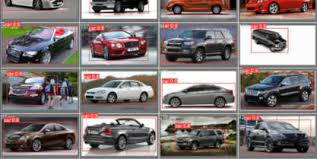
\includegraphics[width=0.85\linewidth]{Figures/Chapter 3/dataset_wotr.png}
    \caption{Một số hình ảnh minh họa và Bounding Box đã được gán nhãn từ tập dữ liệu WOTR}
    \label{fig:dataset_wotr}
\end{figure}

\subsection{Tiền xử lý và tăng cường dữ liệu (Data Augmentation)}
Để đảm bảo mô hình YOLO26 hoạt động tối ưu trên các kích thước đầu vào khác nhau từ thiết bị di động, dữ liệu được tiền xử lý bằng kỹ thuật Letterboxing. Kỹ thuật này sử dụng hàm \texttt{resize\_keep\_aspect} kết hợp với \texttt{pad\_to\_square} nhằm thay đổi kích thước ảnh về chuẩn $640 \times 640$ pixel mà không làm thay đổi tỷ lệ khung hình (Aspect Ratio), giúp bảo toàn các đặc trưng hình học cốt lõi của vật thể cản đường.

\section{Kiến trúc tổng thể của hệ thống SmartNav}

\subsection{Phân tích yêu cầu hệ thống}
Hệ thống được thiết kế hướng tới khả năng xử lý thời gian thực (Real-time). Đối với người khiếm thị, một độ trễ nhỏ trong việc phát ra cảnh báo có thể dẫn đến nguy cơ va chạm vật lý. Do đó, yêu cầu đặt ra là hệ thống phải duy trì tốc độ khung hình (FPS) ổn định, phân tách rõ ràng luồng xử lý giao diện hiển thị và luồng tính toán các mô hình trí tuệ nhân tạo nặng.

\subsection{Sơ đồ khối hệ thống}
Để giải quyết bài toán trên, SmartNav áp dụng kiến trúc Client-Server (Khách - Chủ) chia thành hai khối độc lập hoạt động song song.

\begin{figure}[H]
    \centering
    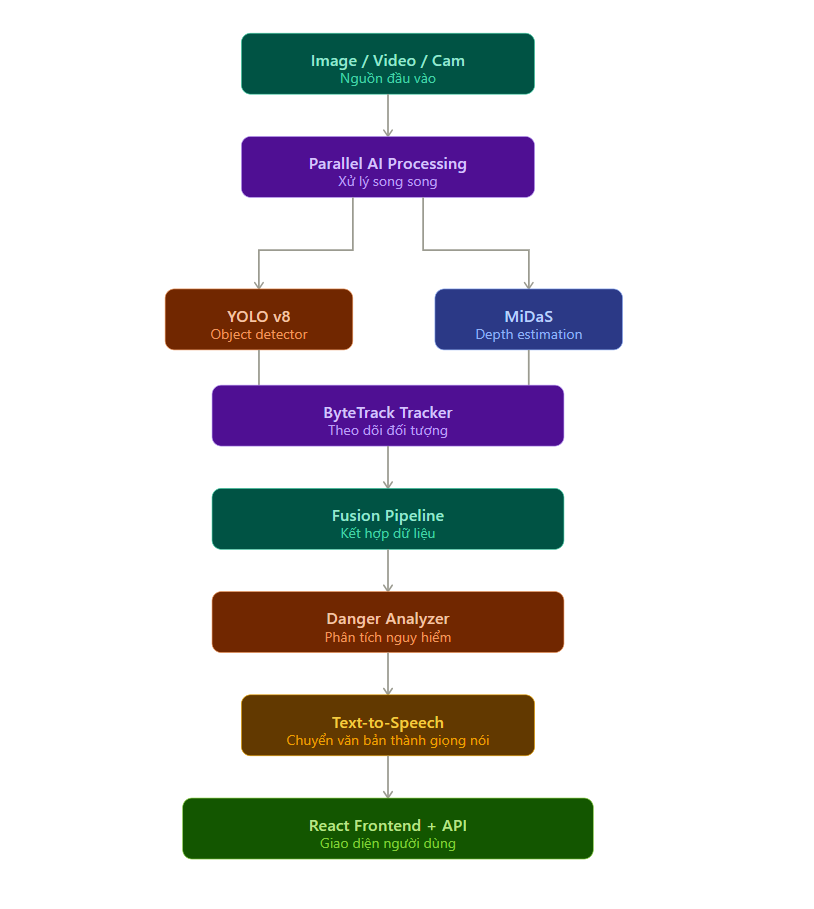
\includegraphics[width=1.0\linewidth]{Figures/Chapter 3/system_architecture.png}
    \caption{Sơ đồ kiến trúc tổng thể và luồng truyền tải dữ liệu hệ thống SmartNav}
    \label{fig:system_architecture}
\end{figure}

Client (ứng dụng Web xây dựng bằng React) chịu trách nhiệm thu thập luồng video liên tục từ Camera, nén và đẩy qua mạng. Server (xây dựng bằng FastAPI) đóng vai trò trung tâm phân tích, tiếp nhận khung hình và chia luồng chạy song song hai mô hình YOLO26 và MiDaS. Dữ liệu sau đó được tổng hợp tại Danger Analyzer trước khi trả về Client.

\section{Xây dựng Khối Trí tuệ Nhân tạo (AI Pipeline)}

\subsection{Nhận diện vật cản với YOLO26}
Việc tích hợp YOLO26 loại bỏ hoàn toàn quá trình NMS (Non-Maximum Suppression) và thuật toán DFL (Distribution Focal Loss) như đã phân tích ở Chương 2, giúp quá trình suy luận (Inference) giảm thiểu chi phí tính toán CPU. Mô hình trực tiếp xuất ra tọa độ khung bao và điểm tin cậy (Confidence Score). 

\subsection{Ước lượng chiều sâu và Kỹ thuật Fallback}
Với mô hình MiDaS, sau khi dự đoán được bản đồ thị sai (Disparity Map), thuật toán sẽ sử dụng mặt nạ Bounding Box do YOLO26 cung cấp để trích xuất không gian độ sâu của từng vật thể. Thay vì tính trung bình toàn vùng (dễ bị nhiễu do nền phía sau), hệ thống áp dụng kỹ thuật Bách phân vị thứ 80 (80th Percentile) để cô lập bề mặt lồi lên gần camera nhất:

\begin{lstlisting}[language=Python, caption={Kỹ thuật lọc nhiễu chiều sâu bằng bách phân vị}]
region = depth_map[y1:y2, x1:x2]
# Trích xuất bách phân vị thứ 80 để đại diện cho bề mặt chướng ngại vật
score = float(np.percentile(region, 80))
\end{lstlisting}

Bên cạnh MiDaS, hệ thống cung cấp phương pháp dự phòng (Depth Fallback) dựa trên Tỷ lệ diện tích khung bao so với toàn khung hình nhằm đảm bảo tính chịu lỗi (Fault tolerance) khi tài nguyên phần cứng bị giới hạn.

\subsection{Theo dõi quỹ đạo (Centroid Tracking)}
Để dự đoán hướng di chuyển của phương tiện, thuật toán Tracking tính toán sự thay đổi tọa độ tâm hình học xuyên suốt tối đa 6 khung hình gần nhất. Bằng cách lấy trung bình sự dịch chuyển trên trục tung ($\Delta y$) và trục hoành ($\Delta x$), hệ thống xác định được vật cản đang tiến lại gần (Approaching) hay ra xa (Receding):

\begin{lstlisting}[language=Python, caption={Phân tích véc-tơ chuyển động xác định hướng}]
avg_dy = np.mean([d[1] for d in deltas])
avg_dx = np.mean([d[0] for d in deltas])
# Vật thể tiến lại gần camera sẽ làm kích thước Bbox tăng, trục Y thay đổi
if avg_dy > 3:
    direction = "approaching"
elif avg_dy < -3:
    direction = "receding"
\end{lstlisting}

\section{Khối Đánh giá Nguy hiểm (Danger Fusion Engine)}

\subsection{Ma trận trọng số và Thuật toán Danger Score}
Module Fusion Engine tổng hợp dữ liệu từ YOLO, MiDaS và ByteTrack để lượng hóa mức độ rủi ro thành Điểm số Nguy hiểm (Danger Score). Thuật toán áp dụng hệ số tổng có trọng số:
\begin{equation}
    Score = (W_{obj} \times 0.4) + (W_{dist} \times 0.3) + (W_{speed} \times 0.2) + (W_{dir} \times 0.1)
\end{equation}

Trong đó, các tham số tĩnh được định nghĩa nghiêm ngặt: $W_{obj}$ (Xe tải = 1.0; Ổ gà = 0.70; Biển báo = 0.25); Khoảng cách rất gần = 1.0; Di chuyển cực nhanh = 1.0; Đang tiến trực diện = 1.0. 
Kết quả đầu ra được phân nhóm làm 4 cấp độ cảnh báo: \textbf{LOW} (An toàn), \textbf{MEDIUM} (Chú ý), \textbf{HIGH} (Nguy hiểm) và \textbf{CRITICAL} (Khẩn cấp).

\begin{table}[H]
    \centering
    \begin{tabular}{|c|c|p{7cm}|}
    \hline
    \textbf{Cấp độ} & \textbf{Ngưỡng Điểm} & \textbf{Kịch bản Xử lý} \\ \hline
    LOW & $< 0.30$ & Hiển thị viền xanh, không phát cảnh báo \\ \hline
    MEDIUM & $0.30 - 0.54$ & Phát tần số âm thanh thấp, cảnh báo có chướng ngại vật \\ \hline
    HIGH & $0.55 - 0.77$ & Phát cảnh báo đỏ, đọc rõ tên và hướng đi của xe cộ \\ \hline
    CRITICAL & $\ge 0.78$ & Báo động khẩn cấp tần số cao, yêu cầu người dùng dừng lại \\ \hline
    \end{tabular}
    \caption{Bảng phân loại ngưỡng điểm nguy hiểm và kịch bản cảnh báo}
    \label{tab:danger_levels}
\end{table}

\section{Xây dựng Giao tiếp mạng và Giao diện Người dùng}

\subsection{Luồng truyền tải WebSocket}
Nhằm tối ưu hóa băng thông, Client không truyền tải video định dạng thô. Luồng Camera (\texttt{<video>}) được trích xuất và vẽ lên \texttt{<canvas>}. Tại đây, thuật toán sử dụng hàm \texttt{requestAnimationFrame} để giới hạn việc lấy mẫu ở mức 5 FPS, sau đó nén khung hình dưới dạng Blob JPEG (quality = 0.7) trước khi đẩy vào đường ống WebSocket:

\begin{lstlisting}[language=JavaScript, caption={Ép khung hình và nén JPEG tại Client}]
canvasEl.toBlob((blob) => {
  if (blob && wsRef.current?.readyState === WebSocket.OPEN) {
    blob.arrayBuffer().then((buf) => wsRef.current.send(buf))
  }
}, 'image/jpeg', 0.7)
\end{lstlisting}

\subsection{Hệ thống cảnh báo đa kênh: HUD và Web Audio API}
Giao diện trực quan áp dụng phong cách hiển thị HUD (Heads-Up Display) hiện đại. Tọa độ của các chướng ngại vật được đánh dấu bằng góc viền (Corner Box) và bảng dữ liệu RadarPanel, đổi màu cảnh báo từ Xanh sang Đỏ tùy theo mức độ \texttt{Danger Score}.

\begin{figure}[H]
    \centering
    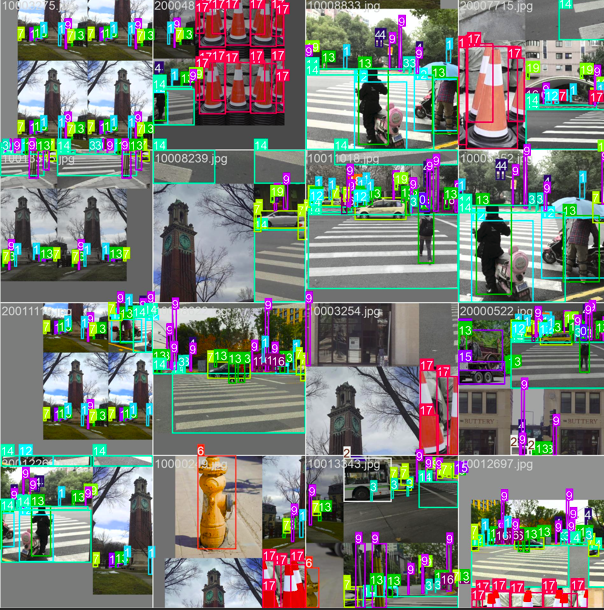
\includegraphics[width=1.0\linewidth]{Figures/Chapter 3/web_interface.png}
    \caption{Giao diện hiển thị trực quan HUD thời gian thực của SmartNav}
    \label{fig:web_interface}
\end{figure}

Cuối cùng, bên cạnh việc sử dụng Text-to-Speech (gTTS) để đọc rõ tên vật cản bằng tiếng Việt, hệ thống áp dụng \textbf{Web Audio API} để kích hoạt tín hiệu báo động độc lập. Bằng cách khai báo bộ tạo sóng \texttt{AudioContext}, hệ thống sinh ra các tần số thay đổi linh hoạt (từ tiếng bíp 440Hz ở mức LOW đến chuỗi báo động giật cục 1000Hz ở mức CRITICAL), tạo phản xạ có điều kiện ngay lập tức cho người khiếm thị trước khi câu nói TTS kịp xử lý xong.

Chi tiết mã nguồn của Backend và Frontend được liệt kê đầy đủ tại Phụ lục B.